% vim:set textwidth=100:
% vim:set fo+=t:

\documentclass[12pt]{article}

\usepackage{amsmath}
\usepackage[nofiglist,notablist]{endfloat}
\usepackage[usenames,dvipsnames]{color}
\usepackage{color}
\usepackage{authblk}
\usepackage{graphicx}
\usepackage{palatino}
\usepackage[activate={true,nocompatibility},final]{microtype}
\usepackage[super,sort&compress]{natbib}
\pagenumbering{arabic}
\parskip = 0.08in \parindent = 0.0in

% Custom macros for author comments
\newcommand{\Alberto}[1]{\color{ForestGreen}#1\normalcolor }
\newcommand{\Justin}[1]{\color{blue}#1\normalcolor}
\newcommand{\Arijit}[1]{\color{magenta}#1\normalcolor}
\newcommand{\Ken}[1]{\color{red}#1\normalcolor}

\author{Arijit~Roy}
\author{Alberto~Perez}
\author{Ken~A.~Dill}
\author{Justin~L.~MacCallum}
\affil{Laufer Center for Physical and Quantitative Biology\\
    and Departments of Physics and Chemistry\\
    Stony Brook University\\
    Stony Brook, NY 11794-5252.}

\title{Predicting the conformational preferences of proteins using a physics-based free energy
method}

\begin{document}

\maketitle

\begin{abstract}

Calculation of free energy differences is of central importance in the simulation of biochemical
systems. It is particularly difficult to calculate between pairs of macromolecular conformations as
well as a computationally expensive task with existing methods. In this work, confinement approach
is used to calculate absolute free energies of biomolecular systems. This method provides two main
advantages: it does not require a reaction coordinate or transition path and it is fast to compute.
Free energy calculated can be decomposed into a per residue contribution in an approximate way. Per
residue free energy allows us to identify the reason behind conformational preferences in
biomolecules. Through out the article we show its use in different challenging modeling problems. In
particular, we show its use in predicting the conformational preference of chamaleon sequences
(sequences with high sequence identity and different folds). This sequence dependent conformational
preferences and per residue free energy decomposition set the stage for the use of this method in
protein design.

\end{abstract}

\Ken{[Guys - I recommend we get a better name than confinement.  It's totally uninformative.  In my view, better would be `confine-and-configure' or something.  
Please give it some thought.]}


\section{Introduction}

In some problems of protein science, you want to know the relative stability of a protein's conformation $A$ compared to it's 
conformation $B$.  We call this the \emph{difference free energy} (DFE). For example, in allosteric mechanisms, a protein often 
adopts one conformation when a ligand is bound and another conformation when no ligand is bound \cite{Elber2007}. To understand the mechanism requires knowledge 
of the relative free energies of the protein conformations.  Another example is in protein structure prediction, for example as practiced in 
the CASP competition \cite{Moult2011}.  If you are using some computational model and have predicted two putative native structures, $A$ 
and $B$, you want to compute which has the lower free energy, in order to know which is the more native-like.  In a third example, you may 
want to know whether mutating a few amino acids in a protein could cause the protein to switch from one stable conformation to another, because 
that could have important consequences for biological mechanisms and disease.  And fourth, sometimes binding a ligand induces a protein from 
one conformation to another.  A quantitative understanding of such \emph{induced-fit} situations requires knowledge of the difference free 
energy of the protein in the two states. In all these cases, it would be useful to have a computational method that can be used efficiently 
with atomically detailed physical forcefield models to compute the free energy differences between different given protein conformations.

Methods like thermodynamic integration \cite{Tironi1994},\cite{Meirovitch2007} which are successful in alchemical free energy calculation
may not be as useful for calculation of conformational free energy.
One widely explored strategy is to use molecular dynamics simulations along some putative reaction coordinate pathway from conformation $A$ 
to $B$ \cite{Elber2007,West2007,Haas2007,Jonsson1998,E2007,Dellago2002,Cheng2006}. \Ken{we need 
many refs here: cite Elber's milestoning, Jhih-Wei Chu, and the many other path-sampling approaches.]} The free energy along this reaction 
coordinate can then be determined using methods such as umbrella sampling \cite{Torrie1977}. Such approaches have several limitations.  
First, it is necessary to know a reaction pathway from $A$ to $B$. If conformations $A$ and $B$ are quite different, then it can be 
challenging to find such paths. Second, these methods 
are computationally slow. To get an accurate estimate of the total free energy difference $\Delta G = G_B - G_A$ requires accurate determinations 
of the many small free energy differences $A \rightarrow 1 \rightarrow 2 \ldots \rightarrow B$, so each microstep requires substantial amounts 
of sampling.  And third, these methods are prone to large errors, because the pathway error is a sum of many errors among the many microsteps.

\Arijit{Will it be useful to add methods like PMF or replica exchange based free energy methods ?}


\Ken{[Are all these methods below ones that don't involve paths?  Also, are there other key methods we should cite?  We need a good scholarly 
list of all the relevant works.]} 
The calculation of protein conformational free energy has been successfully attempted by a number of
groups \cite{Shell2010,Ytreberg2006,Zheng2008,Spichty2010,Strajbl2000,Park2008,Tyka2006,Cecchini2009,Ovchinnikov2013}. 
Some of these methods like reference system method \cite{Ytreberg2006}, deactivated morphing \cite{Park2008}, confinement 
method \cite{Tyka2006,Cecchini2009,Ovchinnikov2013} take an alternative strategy for computing difference free energies 
that does not require knowing a pathway from $A$ to $B$.  
\Ken{[please add the several new Karplus papers from 2012-2013.]}.

Here, we adopt the confinement method of Tyka et al \cite{Tyka2006} and Cecchini et al.\cite{Cecchini2009}. This method 
also resembles the `confine-and-release' method \cite{Mobley2007}, \cite{Mobley2012}, \cite{Mobley2006}.  
\Ken{[cite mobley's jctc 07 (ref 216 on our labsite), and mobley's recent j chem phys review, 
and mobley (ref 199) j chem phys, and others that are relevant.]}. The method is based on the thermodynamic cycle showns in 
Figure \ref{fig:method}.  To start, conformation $A$ is an ensemble.  We reduce ensemble $A$ to one particular microstate $A^\ast$ 
in that ensemble by applying restraints in an MD simulation.  In the same way, we reduce conformational ensemble $B$ to one of its 
microstates, $B^\ast$.  Then, we simply compute the free energy difference between the microstates 
as $\Delta G_{A^\ast, B^\ast} = \Delta H_{A^\ast, B^\ast}$ (which is just an enthalpy difference since there is no conformational 
entropy difference between the microstates).  $\Delta H_{A^\ast, B^\ast}$ is readily calculated using normal mode analysis. In 
this way, we can calculate the free energy difference between the two end states without needing to define a physical path or reaction 
coordinate connecting the two states.

\begin{figure}
\begin{center}
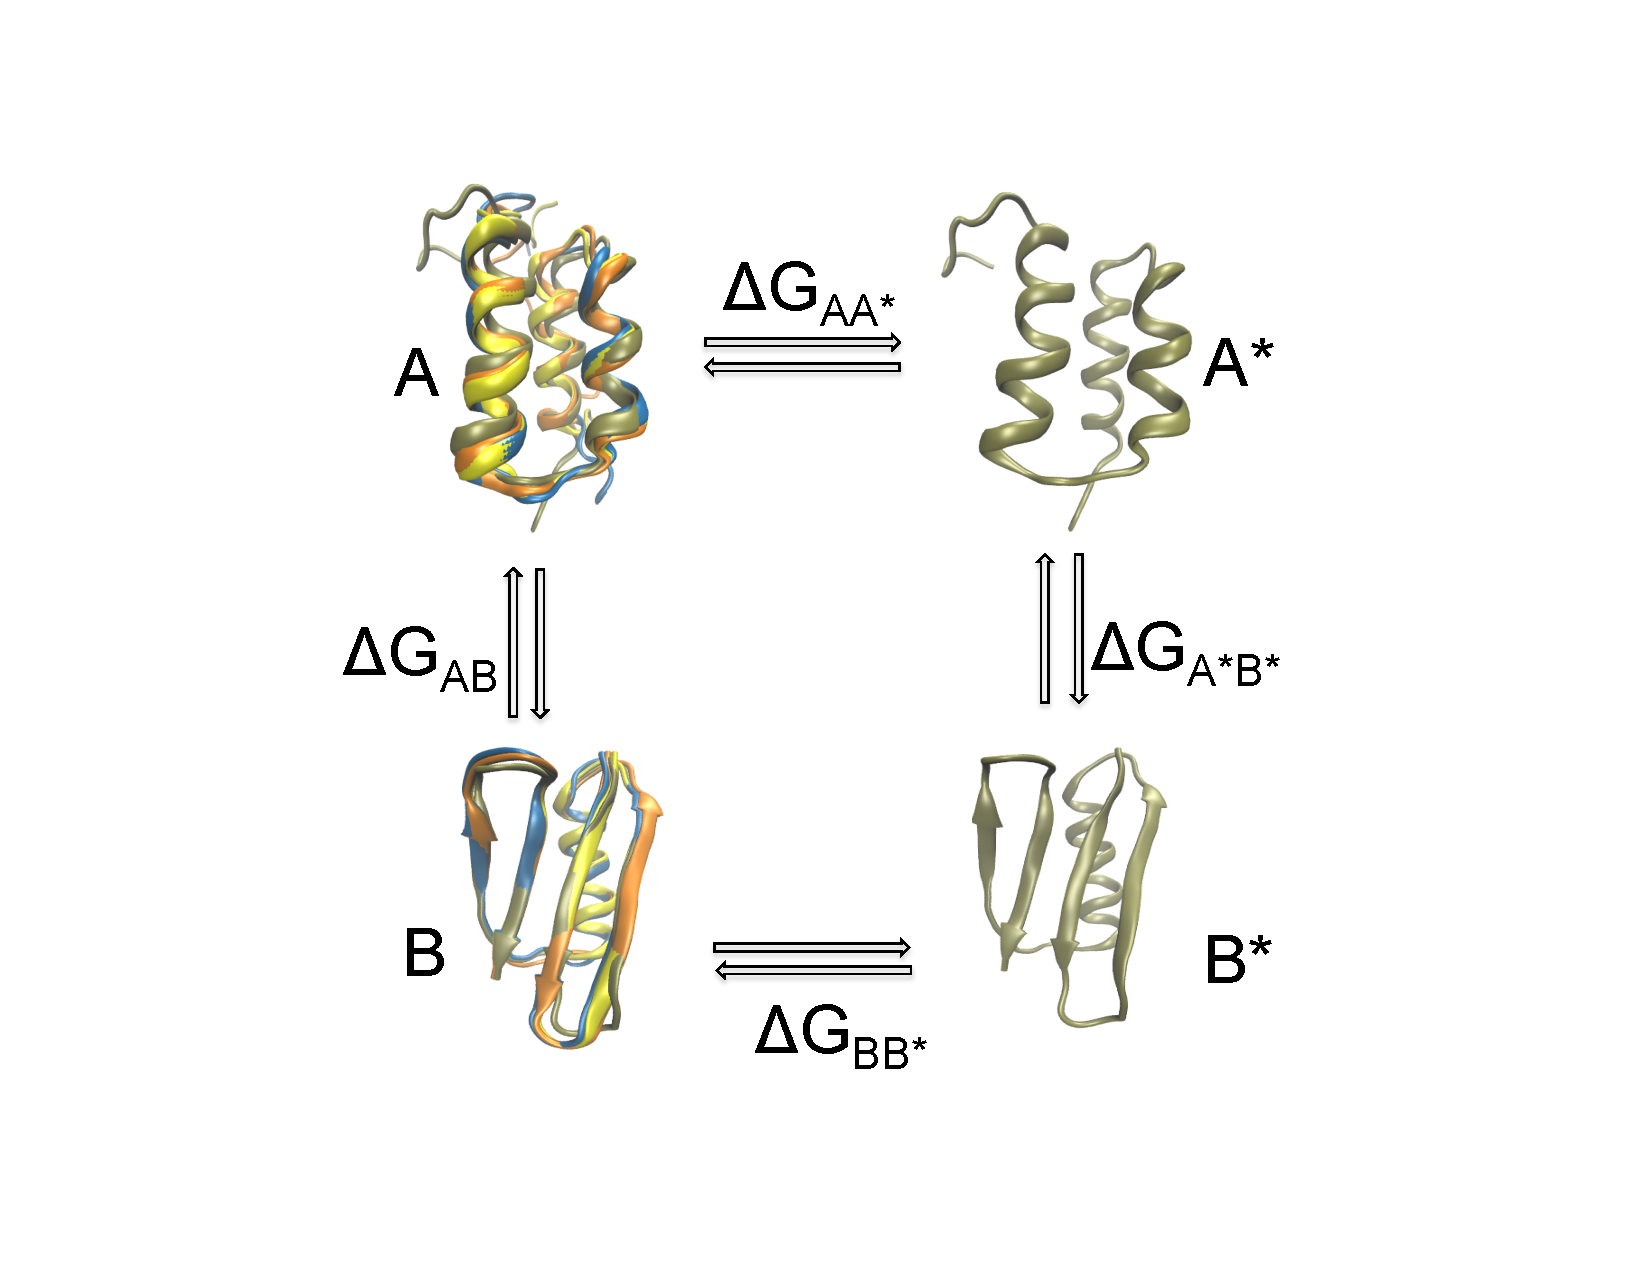
\includegraphics[width=3.5 in,height=3.5 in]{method.pdf}
\end{center}
\caption{Graphical representation of the thermodynamic cycle involving confinement method.}
\label{fig:method}
\end{figure}

\Ken{For this fig, let's make A and A* green and B and B* red or something, to distinguish them visually.  Let's also blur the ensemble more relative to the microstate, so it's clearer the distinction.]}




Previously, the confinement method has been validated on small model peptides \cite{Tyka2006,Cecchini2009}. Here, we show that the confinement 
method can also be applied successfully to larger systems, such as the series of chameleon proteins designed by Orban and co-workers
\cite{Alexander2007,He2008,Alexander2009,He2012}, which can switch between two completely different folds with only few-amino-acid changes 
in sequence.  We also show that our computed difference free energies are useful in evaluating the quality of CASP target protein predictions.  
This could be of significant value for ultimately improving the energetics in protein-structure models, not just the structures.  And, 
finally, we show that we can approximately decompose difference free energies into individual amino acid components.  This offers the 
opportunity for diagnosing the structural basis for difference free energies, which can be useful for interpreting biological mechanisms. 

\section{Results and Discussion}

\subsection{The confinement method succeeds at some basic consistency checks}

First, we validated that our implementation of the confinement method produces results compatible with previous calculations reported in the 
literature.  The method has previously been applied to a 16 amino acid residue $\beta$-hairpin from protein G, known as 
BHP \cite{Cecchini2009}. We calculated the free energy difference between the native conformation (called bhp1), which has 
a two-stranded $\beta$-sheet and a three-stranded $\beta$-sheet called bhp3.  Our confinement calculation shows that bhp1 
is more stable by 1.7 kcal/mol, consistent with 4 $\mu$s equilibrium simulations showing that bhp1 is more favorable configuration 
by 1.8 kcal/mol, and in agreement with previous calculations \cite{Cecchini2009}.

Second, we looked at 6 target proteins from the CASP9 experiment.  For each target, we examined up to 5 submitted models.  We 
computed the difference free energy between the true native and the best model.  Table~\ref{table:casp_control} shows that, in 5 
out of 6 cases, the confinement method assigns a lower free energy to the experimentally determined structure than to any of the 
decoys.  Other well-known discriminators  can also successfully make this recognition \cite{Sheffler2009}; 
 it is just an independent useful validation that the confinement calculations make sense. 

\begin{table}
\begin{center}
\caption{The confinement method assigns a more favorable free energy to the experimentally
    determined structure than to computer-generated predictions. For each target, we examined as
    many as five predictions submitted by CASP participants. We report the free energy difference
    between the most favorable decoy and the experimentally determined structure. Positive
    $\Delta\Delta G$ values indicate that the experimental structure is predicted to be more
favorable than any of the decoys.}
\label{table:casp_control}
\begin{tabular}{l l l}\hline
    CASP Target  & PDB Identifier & $\Delta \Delta G = G_{best~decoy} - G_{native}$ (kcal/mol) \\ \hline
     T0531       &    2KJX        &          $11.15 \pm 0.70$ \\ \hline
     T0538       &    2L09        &          $-3.00 \pm 0.47$ \\ \hline
     T0540       &    3MX7        &          $16.94 \pm 0.49$ \\ \hline
     T0559       &    2L01        &          $2.10 \pm 0.24$ \\ \hline
     T0560       &    2L02        &          $18.00 \pm 0.49$ \\ \hline
     T0569       &    2KWY        &          $20.01 \pm 0.69$  \\ \hline
\end{tabular}
\end{center}
\end{table}

\Ken{[ I think a better notation is $\Delta \Delta G = G_{best~decoy} - G_{native}$, rather than having the arrow.]}

\subsection{The confinement method correctly predicts the structures of chameleon sequences}

We also tested the confinement method predictions for difference free energies on the chameleon sequences of Orban 
et al. \cite{Alexander2007,He2008,Alexander2009,Bryan2010,He2012,Shortle2009}; these 
are instances in which two highly similar sequences fold into remarkably different structures. Orban and co-workers have designed a 
protein-G-like sequence of 56-residues that
is marginally stable in one of two possible folds. By mutating key residues in this sequence they
are able to stabilize one fold or the other (see Figure~\ref{fig:orban}). We call sequences ``$\beta$'' that fold into 
the protein-G-like that fold into a $4 \beta + \alpha$ fold, and we call sequences ``$\alpha$'' that fold into $3 \alpha$ helical folds.  One pair 
of sequences (GA88/GB88) is 88 percent identical in sequence, differing in seven positions. Another pair (GA95/GB95) is 95 percent identical, 
differing in three positions. The third pair (GA98/GB98) differs in only a single tyrosine-to-alanine mutation. Accurately predicting the 
structural preferences of these structures presents a serious challenge for computational methods 
\cite{Alexander2007,He2008,Alexander2009,Bryan2010,He2012,Shortle2009}.

\begin{figure}
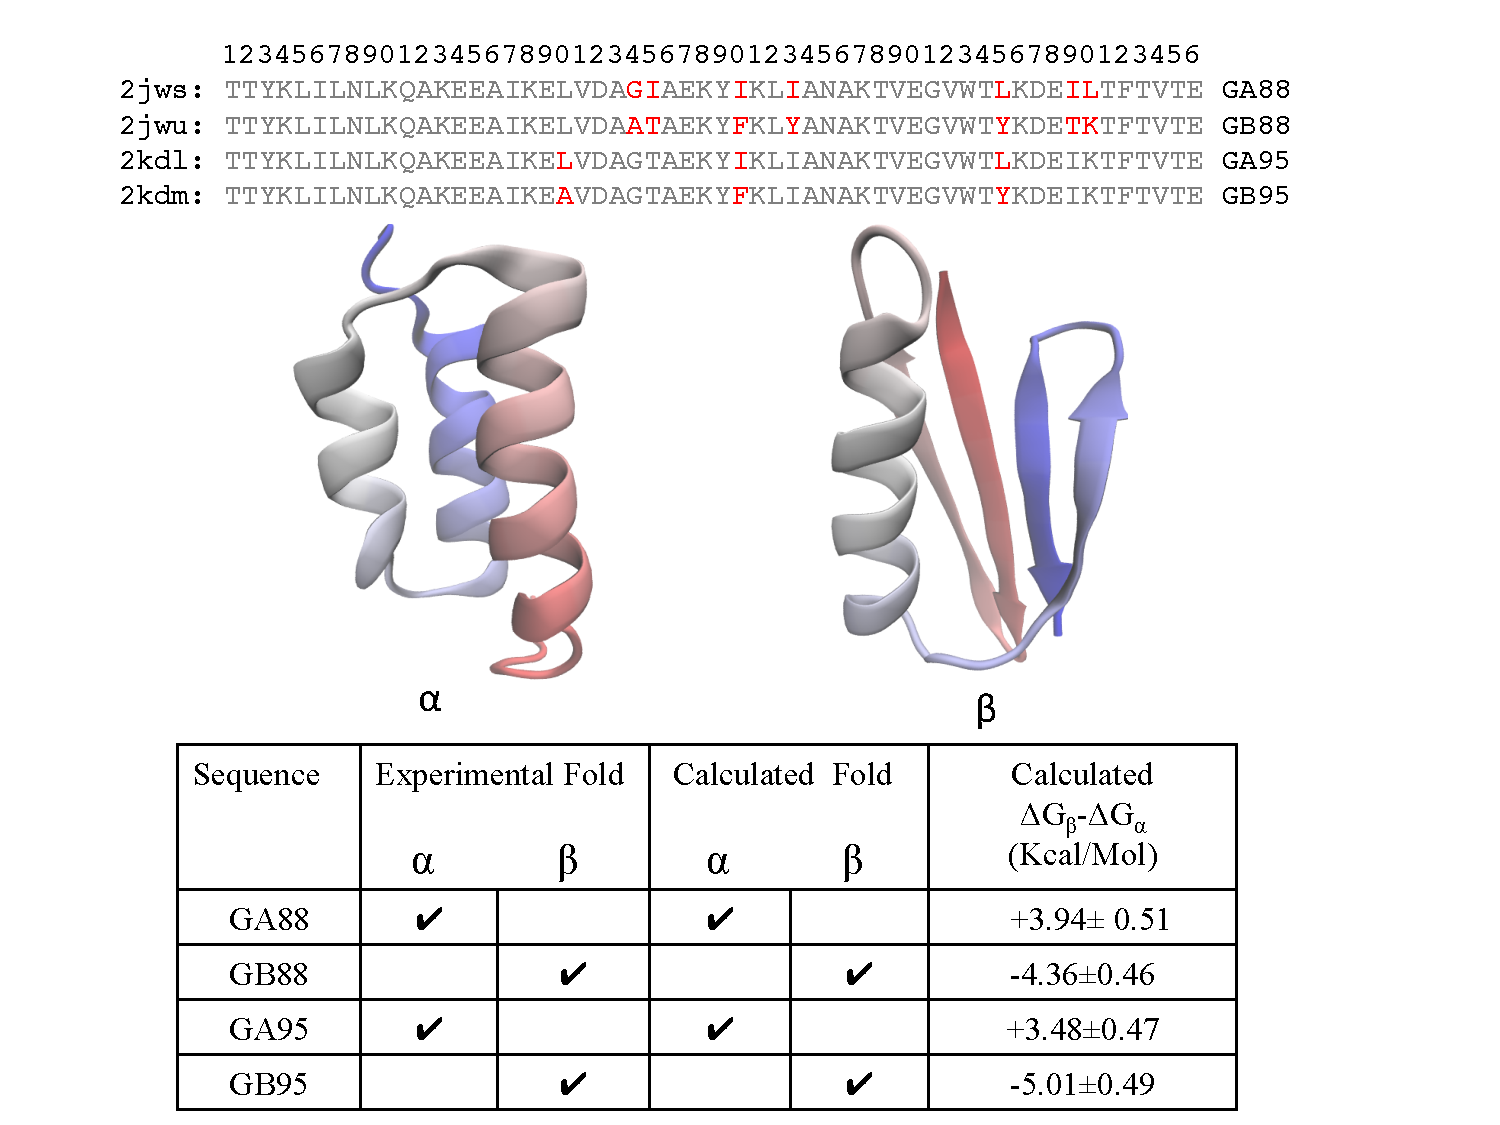
\includegraphics[width=5.0in]{orban.pdf}
\label{fig:orban}
\caption{Confinement method correctly predicts the structural preferences of four chameleon
sequences. The top part of the figure represent four sequences used in this study along with the
protein data bank id. Each sequence adopts either a three-helix bundle fold (denoted $\alpha$) or
$4 \beta + \alpha$ fold (denoted $\beta$). The relative free energies of
the two folds are reported for each sequence.}
\end{figure}

We initially approached this problem by making a model of each sequence with the same backbone
structure as its partner chameleon sequence. For example, we took the sequence of GA88 and built a
model with the same overall structure as GB88. We then used the confinement method to assess the
free energy difference between the experimentally determined structure of GA88 and the model (with
the GA88 sequence and the GB88 structure). The confinement method was able to predict the
conformational preferences correctly for all four sequences (data not shown). This is, however, not
surprising. It is well known [CITE]\Arijit{still searching this citation} that it is easy to distinguish 
computational models from native structures. To avoid this potential problem, we instead computed relative free energy of two
different computer generated models for each sequence. One model is based on the $\alpha$ structure and
the other on the $\beta$ structure (see Supporting Information for details on the modeling procedure).
This is a much more realistic test of the confinement method's ability to accurately calculate
relative free energies. 
 
\Ken{[ It's not clear what this test is and why it's better, and why there are only 5 sequences.  Please clarify.]}
\Arijit{ Now there are 4 sequences as they have the experimentally available structure. The fifth sequence is discussed 
at the end of the paragraph.}


Figure~\ref{fig:orban} shows that the confinement method identifies the correct structure for all four sequences. One hypothesis for fold switching of
chameleon sequences is that the structural transitions require states with diminished stability
\cite{Bryan2010}. It is believed that if the free energy of the native state and the alternative state are
within a range of 5 kcal/mol, then it is possible for the native state to be destabilized relative
to the alternative state with only small changes in sequence. The stability of the native state can
decrease for a number reason ranging from chemical modification, breaking of disulphide bonds or
mutations---as is the case here. The calculated free energy differences range from around 3.5 to 5.0
kcal/mol, which is consistent with the above hypothesis \cite{He2008,Alexander2009,Bryan2010}. 
In a more recent study\cite{He2012}, the amino acid residue at position 45 (Tyr for $\beta$ and Leu for $\alpha$) was
found to be important for switching between  $\alpha$ and $\beta$ conformation. This inspired us to 
introduce another mutation at 45 position. For our future reference this Tyr-45-Ala mutation of GB95 sequence will
be known as GB98. Interestingly, with this mutation, the equilibrium shifts to $\alpha$ conformation as it gains 3.84 Kcal/Mol 
stability compare to $\beta$ conformation and indicate the importance of Tyr-45 residue. It will be interesting to 
know the actutal experimental structure which can validate our result.  

\subsection{Per-residue free energy calculation can identify the mechanistic detail behind
conformational preferences} \label{sec:orban_per_residue}

To understand the mechanism behind the conformational preferences of the different protein
sequences, we decomposed the calculated free energy into per-residue contributions in
an approximate way \cite{Tyka2006}. For this purpose, the confinement free energy, $\Delta G_{A,A*}$ and
$\Delta G_{B,B*}$ of each residue is calculated in the usual numerical way as described
the method section. We call this method approximate as we ignore the contribution from the normal 
mode or quasiharmonic analysis. Instead, decomp module of amber is used to calculate the internal energy 
of each residue from the final restrained trajectory. 

\Ken{[Arijit -- I didn't find this methods calculation.  We should at least put in a sentence or two here summarizing it.]}  
This helps us to identify important residues that stabilize a particular
conformation. The per residue free energy, $\Delta \Delta G ((\beta) - (\alpha))$ is
shown in Figure~\ref{fig:perresidue_orban}. 
In this plot, residues colored in blue favor the $\alpha$ structure, residues in red favor the $\beta$ structure, and white residues
have no preference.


\begin{figure}
\begin{center}
\includegraphics[width=4.5in]{delta_g.pdf}
\end{center}
\caption{The $\alpha$ and $\beta$ conformation associated with GA95 and GB95 sequences are colored according to the relative per residue
free energy value. In this figure, residues colored in blue favor the $\alpha$ structure, residues in red favor the $\beta$ structure, and 
white residues have no preference. Some of the mutated residues are also labelled.}
\label{fig:perresidue_orban}
\end{figure}

Although the overall free energy difference between the two structures is small (within 3-5 Kcal/Mol), the individual residues 
can show marked preferences for being in either $\alpha$ or $\beta$
conformation. Such differences can be undestood by looking in detail at the local environemnt for
those resiudes. For example, the region around residue 7 forms a random coil in the $\alpha$
structure, whereas it is forming a beta sheet structure in the $\beta$ structure. These residues
strongly favour the locally well packed and hydrogen bonded environment found in the $\beta$ sheet.
Overall, favoring $\alpha$ or $\beta$ structure is a delicate balance, were the relative global free
energy difference is small and the contributions of different per residue tendencies balance out. It
is therefore very likely that by changing key resiude preferences the global fold preferences can be
changed.

Three residues are mutated between GA95 and GB95, at positions 20, 30, and 45. In GA95, these
residues (L20, I30 and L45) stabilize the $\alpha$ structure. In GB95, two of these residues (F30
and Y45) favor the $\beta$ structure, because they have large solvent exposed surface areas in the
$\alpha$ structure, but are more buried in the $\beta$ structure. Additionally Y45 forms a hydrogen
bond with D47 in the $\beta$ structure. On the other hand, residue A20 from GB95 still favors the
$\alpha$ structure, although not as strongly as L20 in GA95.

The $\alpha$ and $\beta$ sequences are nearly identical, so there are some common features observed for all
sequences. Roles of some important residues in stabilizing either the $\alpha$ or $\beta$
conformation and possible reasons for such conformational preferences are summerized in 
supporting information Figure S1. The experimental observations
classified the protein into two parts: Amino acids 9-51 are fully structured in both folds, whereas
residues 1-8 and 52-56 are unstructured in the $\alpha$ fold, but form a $\beta$-strand in the
$\beta$ fold. Most of the amino acid residues in the region 1-9 have negative per-residue free
energies, which means that these residues favor the $\beta$ structure.

In addition to the direct effects of the mutation, there are also indirect effects due to small
perturbations due to the mutations. For example, the L20A mutation causes a slight repacking around
residue 20. This causes large changes in the per-residue free energies of nearby residues T25 and
A26. However, these differences largely cancel and the overall effect of the L20A mutation is weaker
than either the I30F or L45Y mutations.

Such per-residue free energy decompositions allow us to understand the driving forces behind protein
folding and conformational change and may be useful for designing proteins with specific structures
and functions.

\subsection{Applcation of confinement method for structure prediction}

We applied the confinement method as a ``meta-predictor'' for structure prediction. Here, the
task is to correctly identify the most accurate models out of a set of ``decoys'' generated by
different methods during the Critical Assessment of Structure Prediction (CASP) experiment. CASP is
a blind test in which different groups apply methods to predict the 3-dimensional structure of
proteins from their sequences. Each group is allowed to submit five
possible structures, which they are supposed to rank from best to worst. We have performed two
experiments centered on CASP.

In the first experiment, we examined several targets and tried to rank-order the predictions
made by the same group (same methodology used to generate the models), in others the
structures were drawn from several different groups (different methodology used). The goal of this 
experiment is to determine whether 
the physics-based confinement method can correctly identify more native-like structures as having
low free energies.

Our second experiment was to see if the confinement method can identify structures that are missed
by other meta-prediction servers. Most successful meta-prediction servers are based on the idea of
consensus: if many different prediction methods produce similar results, then that is probably a
correct prediction. This is often a powerful heuristic, but it can miss cases where there is a very
good result that is only predicted by one method. We chose several cases where such structures were
missed and assessed if the confinement method can correctly identify these accurate models.

As is common in the CASP experiment, we assess our results in terms of Global Distance Test Total
Score (GDT-TS) \cite{Zemla2003}, which is a C$\alpha$ based measure of structural accuracy. It can
be understood roughly as the percentage of residues that are correctly positioned in the model
(range 0 to 100, higher is better). The initial models for the test was chosen from different server 
groups those have traditionally done well in past CASP events.

\subsubsection{The confinement method can correctly rank different models generated by the same methodology
and distinguish the native structure}

Here, our task is to rank different submitted models of CASP9 targets that have been generated with
the same methodology. In absence of any other reliable alternative, we compare all our free energy based 
ranking with the GDT-TS based ranking which are available in CASP website.  

The first test case is a protein BVU3908 from Bacteroides vulgatus whose PDB id and CASP target 
code are 2L01 and T0559 respectively.
The best predictor group for this 69 amino acid long target was "BAKER-ROSETTASERVER". We initially checked similarity
between the models submitted by them and discarded two from the analysis on
the basis of being too similar to some of the other models. The GDT\_TS score and rmsd values as
shown in Figure~\ref{fig:T0559} indicate that model 1 was predicted correctly, whereas the order of
model 3 and 5 was wrong. The main difference between model 3 and rest of the models was the  
orientation of the first alpha helix. On the other hand, as shown
in Figure~\ref{fig:T0559} the confinement method not only can differentiate the native
structure from the submitted models, the ranking also correlates perfectly with the GDT\_TS score.  

\Ken{Arijit- we could probably make a better visualization of this figure above by putting it onto a toy landscape: x-axis is rmsd, y-axis is DDG, and above each of the 4 points on this graph will be the ribbon diagram and the GDT-TS.  I suggest we do that with the fig below too.  Let's don't use 4 different colors for the fig below.  Let's just show differences in structures in some different color, or show them all as green.]}

\begin{figure}
\begin{center}
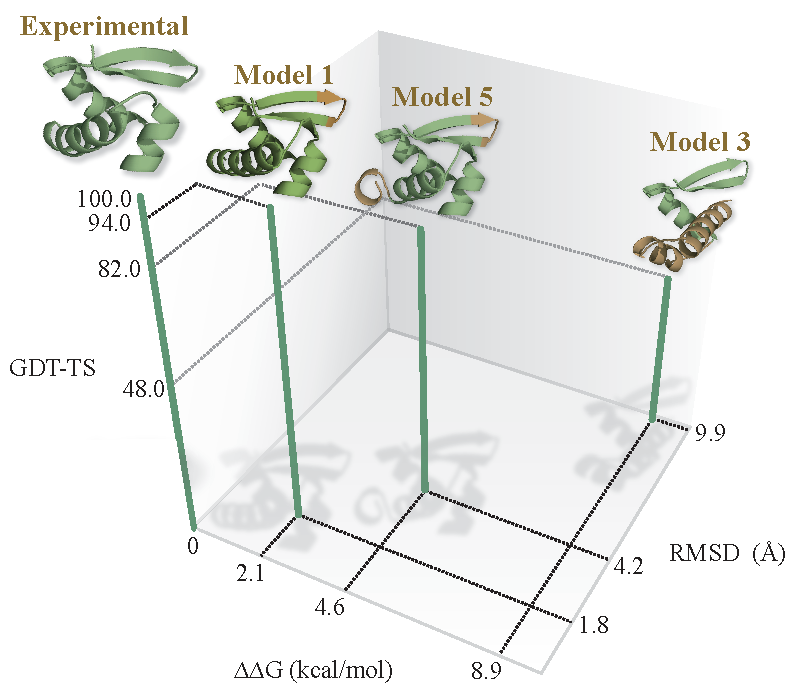
\includegraphics[width=3.8 in,height=3.2 in]{T0559.pdf}
\end{center}
\caption{The native and three submitted model structure, along with their GDT\_TS, RMSD and relative Free energy values
of protein BVU3908 from Bacteroides vulgatus (PDB id: 2L01 and CASP code: T0559).}
\label{fig:T0559}
\end{figure}


To further test the method we continued with the example of protein BT2368 from Bacteroides
thetaiotaomicron. The PDB id of this 74 amino acid residue protein is 2L02 and CASP target code is
T0560. We compared the free energy difference between the native structure and the two of the
five submitted models from the group "Splicer". The remaining three models were discarded as 
they were too similar to the rest of the models. As shown in Figure~\ref{fig:T0560}, we can identify 
the native state correctly and our calculated free energy based ranking matches well with the
GDT\_TS score. 

\begin{figure}
\begin{center}
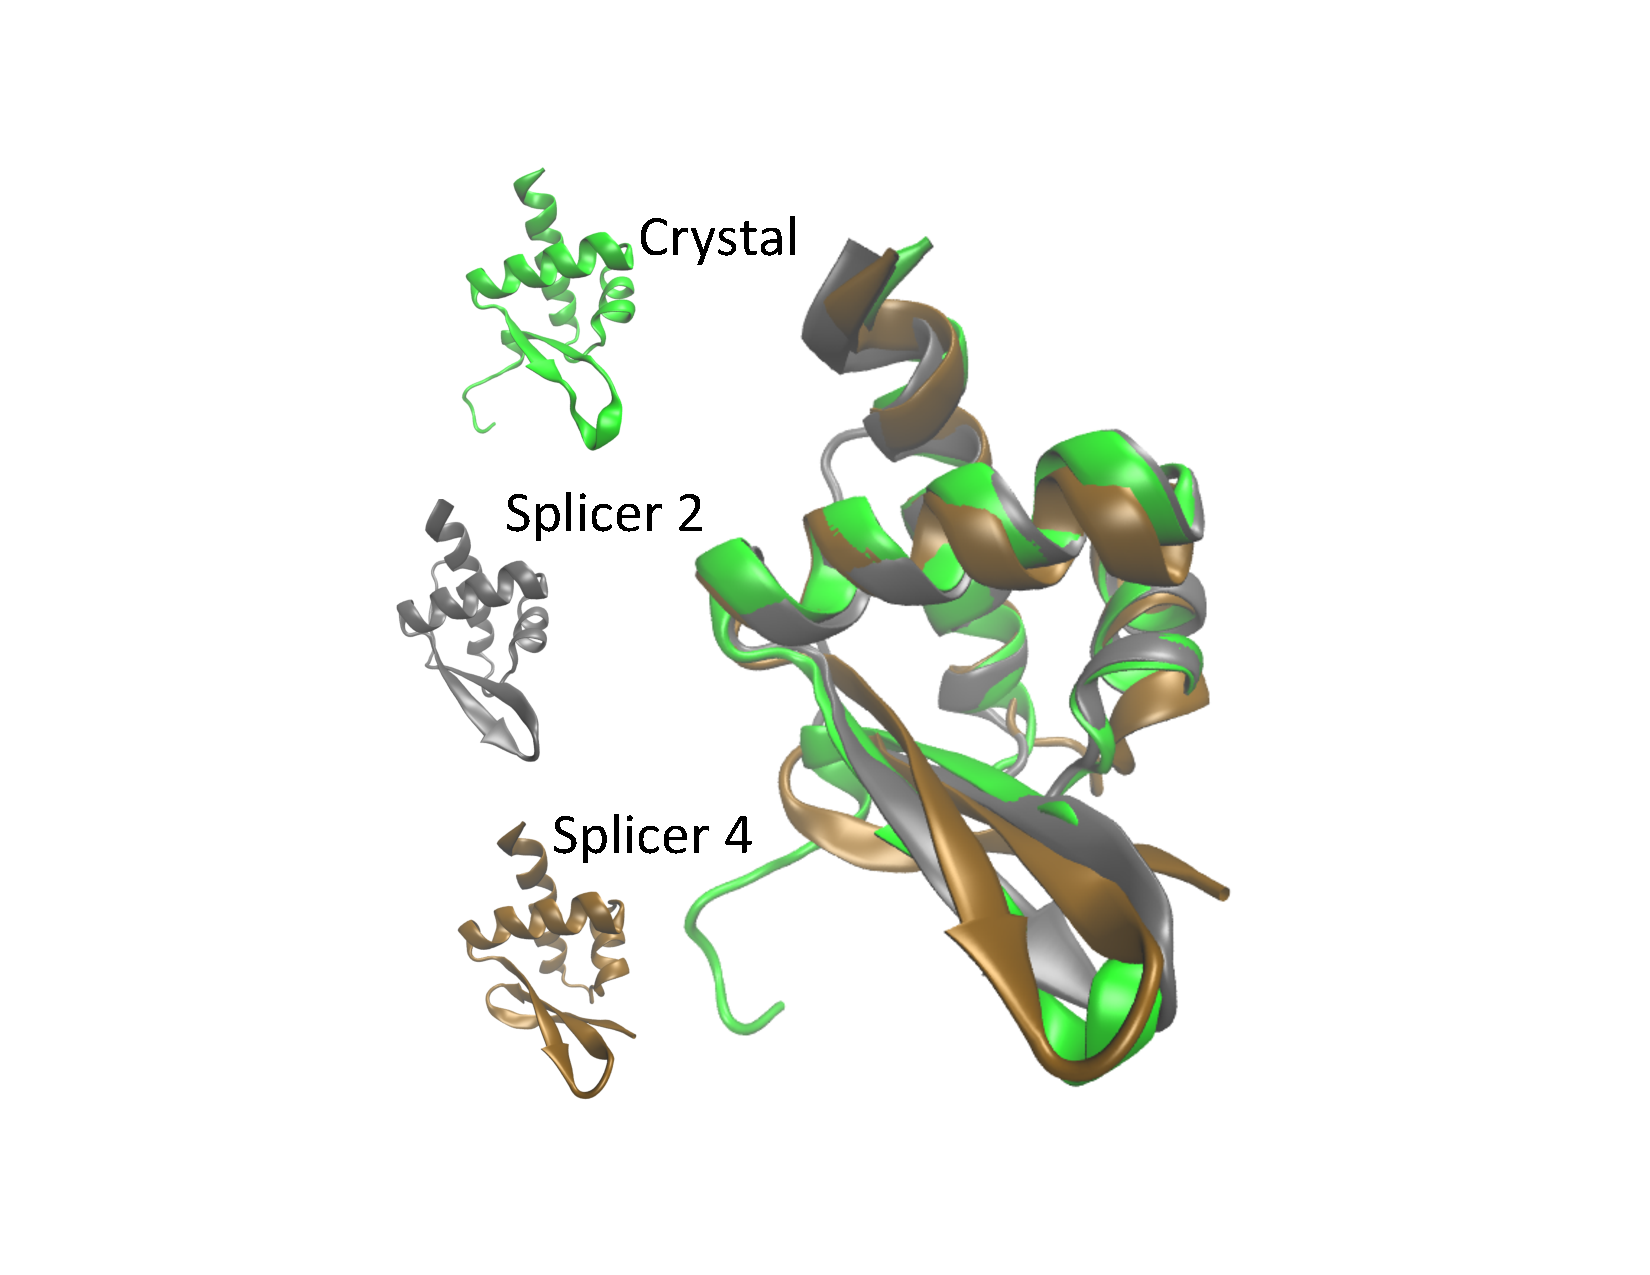
\includegraphics[width=4.0 in,height=3.0 in]{T0560.pdf}
\end{center}
\caption{Native and two model structure of protein BT2368 from Bacteroides thetaiotaomicron (pdb id: 2L02 and CASP code: T0560). The two models
were from the group "Splicer".}
\label{fig:T0560}
\end{figure}


\subsubsection{The confinement method can rank models generated by different methods}

Our next test was between models that are produced with different methodologies. 
Here, our model system was a fas apoptosis inhibitory protein molecule whose
pdb id and CASP target codes are 3MX7 and T0540 respectively. 
This protein contain 8 beta strands and 90 amino acid residues. 
The top models from groups "LTB" and "Mufold" was chosen for analysis.
We will call this as Model 1 and Model 2 for future references. As summerized in
Figure~\ref{fig:T0540}, the free energy based ranking once again correlates well with the 
GDT\_TS based score.

\begin{figure}
\begin{center}
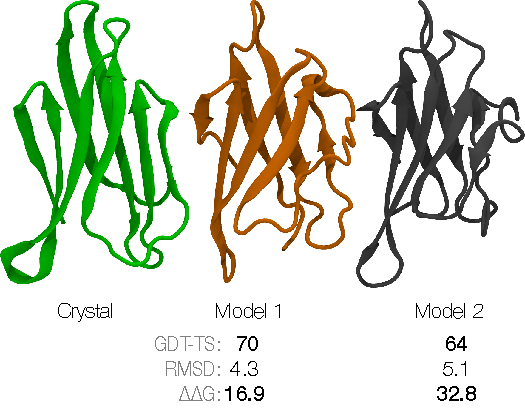
\includegraphics[width=4.0 in,height=3.4 in]{T0540.pdf}
\end{center}
\caption{X-ray crystallographic structure and two submitted models of fas apoptosis inhibitory protein (pdb id: 3MX7 and CASP code: T0540).
Model 1 and Model 2 in this analysis were submitted by the group LTB and MUFOLD respectively.}
\label{fig:T0540}
\end{figure}

\subsubsection{Per residue free energy calculation identifies the residues that are responsible for
differences between two conformations}

\Ken{[Arijit - This and the following sections need to be shortened and made more concise.]}

In section~\protect\ref{sec:orban_per_residue} we discussed how per residue free energy calculation
can identify the mechanistic detail behind conformational preference of a chameleon sequence. In this section, our aim 
is to apply the same method and try to understand whether per residue free energy can help us identify
residues which stabilizes/destabilizes a particular region of a protein. The difference  
here is that the protein has similar fold with only mismatch in some region. 
To investigate this, we choose a domain of adhesion exoprotein from Pediococcus pentosaceus (pdb id=2KYW) from protein data bank 
and its best predicted model of CASP9 (casp id=T0569, submitted by 'Mufold' group which had a GDT\_TS of 78).
We first calculated the free energy of the whole protein and found that the native 
structure is stabilized by 20 Kcal/Mol (see suppurting information Figure S2). 

Next we proceed with the per residue free energy calculation. Our effort clearly identifies two hydrophobic residues 
Val-59 and Ile-61, which destabilizes the submitted model with respect to the crystallograohic structure.
The sidechains of these hydrophobic residues are oriented towards the protein hydrophobic core in the
native NMR structure but oriented outside protein and solvent exposed in the model. These residues are the primary reason
why two of the beta sheets in the native structure are disordered in the model structure ( see Figure~\ref{fig:T0569_per_residue}
and supporting information Figure S3). This method also identifies some other residues which stabilize/destabilize either 
of the conformation. For
example, Lys-76 stabilizes the model as it has a H-bond with Asp-11 which is missing in the native structure
(Figure~\ref{fig:T0569_per_residue} and supporting information figue S3).

\begin{figure}
\begin{center}
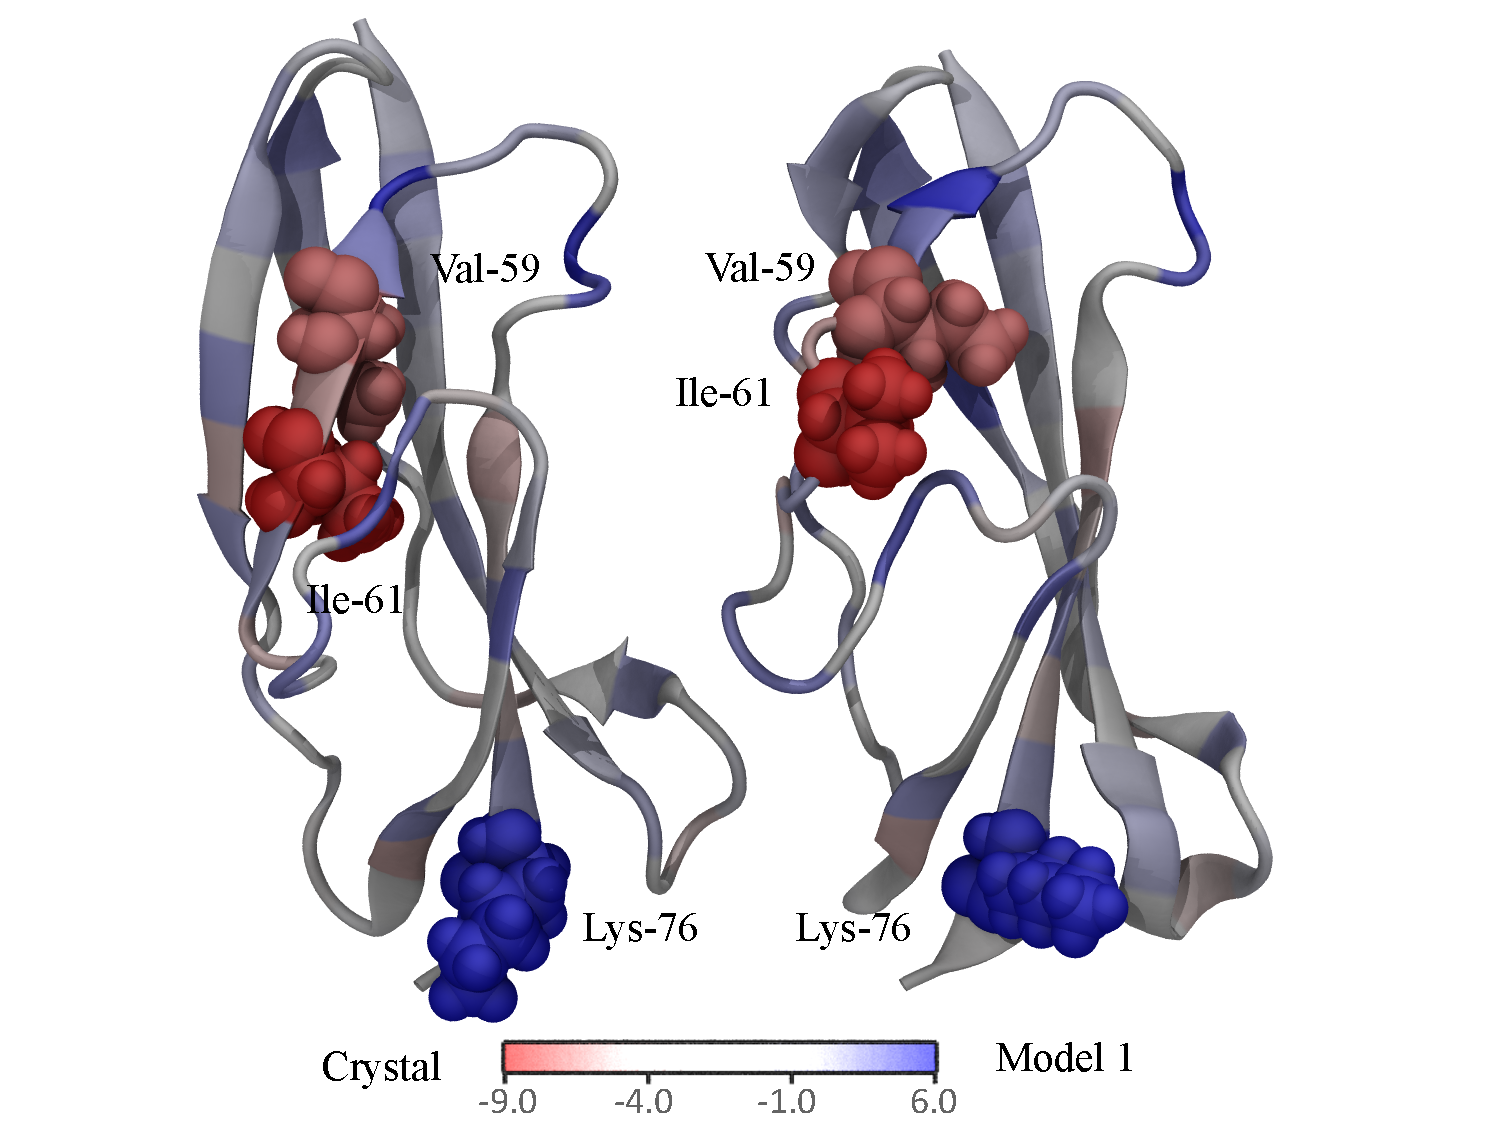
\includegraphics[width=4.3 in,height=4 in]{T0569_perres1.pdf}
\end{center}
\caption{To better understand the reason behind difference in conformation, structure of CASP Target 569 (pdb id: 2KWY) and a 
generated model was colored according to the per residue free energy value. The amino acid residues that are colored in deep red 
and deep blue stabilizes the crystal and the model respectively, while the residues with light blue color does not have a preferance.
 Some of the important residues are also labelled.}   
\label{fig:T0569_per_residue}
\end{figure}

\subsubsection{Failures in the confinement method}

Despite the great success in most of the studied systems, there are few failures, specially when
the GDT scores of the compared structures are very close. We observed this for a $54$ amino acid residue long
 engineered protein from Asr4154 protein (pdb id: 2L09 and CASP code T0538).
Like previous cases, we kept the native structure and include models from the group "PconsR" (GDT\_TS=96.23, model1),
"Shell" (GDT\_TS = 90.09, model2) and "FOLDIT" (GDT\_TS = 86.32, model3) for analysis. 
Contrary to our expectation, model1 was found to be more stable than the crystal structure 
(see Figure~\ref{fig:T0538}). In order to rationalize such obseravtion we calculates per residue free energy
between crystal structure and model1. The results show us that despite the small variation at the backbone level (as
shown by high GDT\_TS scores and low RMSDs), the sidechains are oriented in very different ways,
giving rise to large differences in the stabilization of certain residues. In particular, some of
the differences arise from different salt bridge patterns (Arg-32 with Glu-35, Glu-28 with Lys-24 and Arg-26 with Glu-50
in crystal versus Arg-32 with Glu-28 in model 1) and certain flexible polar residues exposed to the
surface (Lys-24 in model 1, which has an entropic gain from absence of salt bridge and is
stabilized by interactions with the solvent) (See supporting information Figure S4). All in all, this
unexpected result just shows us that this method is sensitive to local interactions such as those
happening from side chain reorientation and also indicate the limitations of GDT\_TS based ranking. 

\begin{figure}
\begin{center}
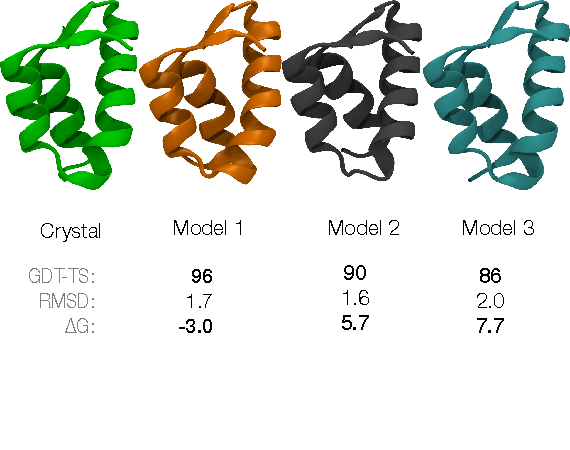
\includegraphics[width=3.6 in,height=3.4 in]{T0538.pdf}
\end{center}
\caption{The native and three model structure of engineered protein from Asr4154 protein (PDB ID: 2L09 and CASP code:T0538). The model 1,2 and 3 are
from the group PconsR, Shell and FOLDIT respectively.}
\label{fig:T0538}
\end{figure}


\subsubsection{What can we say about low resolution models?}

So far we have seen that the method is good at predicting preferences when the structures are not
very far from the native. But the question remains how far from native can we go and still see 
that the method produces correct result. In this section we explored this question with models from  
extracellular domain of the jumping translocation breakpoint protein (pdb id: 2KJX). Most of the
group could only generate low resolution models for this CASP9 target (id: T0531) . In our comparison, we choose five
models by the group MUFOLD-MD, which was the best performing group for this target with their best model 
had a GDT\_TS value of 44. The result presented in Figure~\ref{fig:T0531} shows: 1.) native is correctly identified as
expected and 2.) Surprisingly there is a high level of correlation between the GDT ranking and the
free energy ranking for model 1 and model 3, the rest three structures with GDT\_TS score less than
35  are ordered incorrectly. It is worth to note that models 2 and 3 have the same GDT and very
different free energies, meaning that the actual ordering could change a lot \cite{Perez2012}. It is
encouraging that at least the method can pick out the best model even though it is got a low GDT
score: 44.  

\begin{figure}
\begin{center}
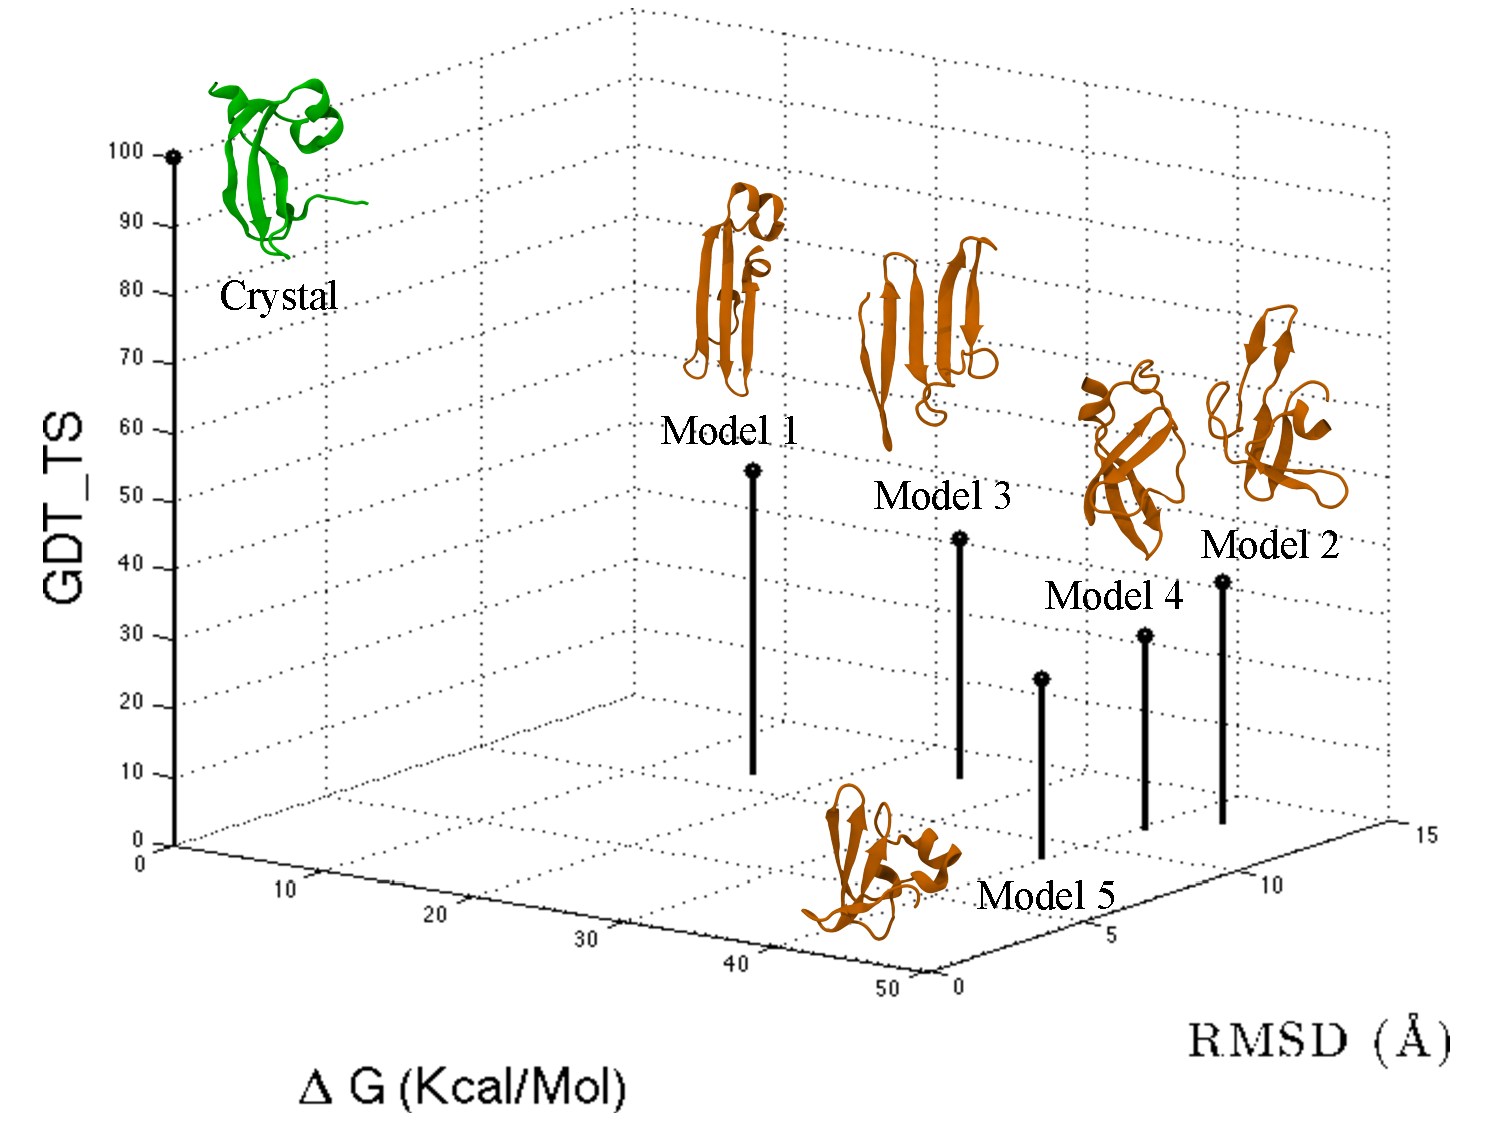
\includegraphics[width=3.5 in,height=3.5 in]{T0531.pdf}
\end{center}
\caption{The native structure and 5 models of extracellular domain of the jumping translocation
breakpoint protein (pdb id: 2KJX and the CASP code: T0531).}
\label{fig:T0531}
\end{figure}

\subsubsection{Can the confinement method perform better quality assessment in protein structure prediction?}

\Ken{[Arijit - let's make the following section more concise and focused.]}

A part of the CASP experiment is dedicated to the quality assessment (QA) of predicted models
\cite{Kryshtafovych2011}. Here, predictors were asked to score each model on a scale 
(known as qmode) from 0 to 1, with higher values corresponding to better models \cite{Kryshtafovych2011}. 
It will be interesting to know how confinement method perform in quality assessment compare to 
the other groups in CASP9. We investigated this using couple of CASP Targets. Here, we present a 
case, where confinement method perform well than the top performing group MUFOLD-WQA \cite{Wang2011} 
of CASP9. We choose  
two models from CASP taget T0538. They were model 3 submitted by PconsR (GDT\_TS = 96, qmode 1 = 0.5434) 
and model 5 from the MULTICOM-NOVEL ( GDT\_TS = 83, qmode 1 = 0.5865). Both are server predicted models and
the qmode value presented are from MUFOLD-WQA \cite{Wang2011}. We choose these two models as
the model by PconsR was the most accurate predicted model for this target, whereas the other model 
was predicted best by QA test of MUFOLD-WQA. The calculated free energy using confinement method indicate
that the model by PconsR is more stable by $3.9 Kcal/Mol$ which support the GDT\_TS trend.
There is no doubt that the consensus approach can predict the model quality
in a faster manner. But we expect confinement method can predict the model quality in a
relatively expensive but much more accurate way.

\section{Conclusion}

We have described a computational method called confinement for computing the difference free energy from a protein conformation $A$ to $B$.  We 
show that it can give accurate values, even for relatively large conformational changes.  We have demonstrated that it can discriminate 
which Orban chameleon peptides fold into a 3-helix bundle vs. a 4$\beta$+1 helix structure. We show that it can discriminate between good and bad CASP 
models.  Perhaps most importantly, we have shown that it can be used to give residue-level insights into what are the dominant structural factors in a 
protein that are responsible for the difference free energies.  A key advantage is that this method does not require any reaction coordinate, or sampling 
a pathway from conformation $A$ to $B$. We have tested the method for structures of proteins having up to 100 amino acids.  The computational cost 
for a 56-residue protein is about 4 hours [on 1 gpu] for 20 ns of confinement [Is 20ns all you need?]. 

\Arijit{I need 21 (confinement run) x 20 ns for single confinement}
%There is another issue, which is normal mode analysis calculations are Oh(N**3) and require large
%amounts of memory, effectively limiting the size of the systems under study. In most cases
%quasiharmonic analysis.  

\Ken{[If this is a relevant limitation, let's say something about it.]}
\Arijit{I think Ken is pointing towards the normal mode issue and number of residues that we can handle}


\section{Method}

The confinement method has been described in details in ref. by Tyka et al. \cite{Tyka2006} and
Cecchini et  al. \cite{Cecchini2009}. The basic approach of the confinement approach is the same in
both these papers. However, there are some technical differences. Here we briefly describe the
procedure to compute free energy $\Delta G_{AB}$ between two conformations A and B of a protein. The
basic idea to compute the free energy between conformations A and B is to perform a thermodynamic
cycle:

\begin{enumerate}

\item  Minimization of A and B. These minimized conformations (A* and B*)
       are the reference conformation of that state. During this minimization the backbone is kept
       restrained to the original position to avoid large conformational changes.

   \item  The free energy of confining the ensemble (A or B) to a microstate (A* or B*) is
       calculated. This is done by gradually applying larger and larger
       harmonic restraints on all the atoms of the biomolecule. This is done by running 21 molecular dynamics simulation 
       (20 ns long each), where the harmonic restraint force constant was scaled from 0.00005
       Kcal/Mol 
       (mostly free) to 81.92 iKcal/Mol (frozen in one microstate). In this final restrained state, the
       rotational contribution to the free energy is frozen out
       and the only remaining contribution is the vibrational part. The free energy for this step is
       estimated from the fluctuations around
       the reference structure using a numerical
       approach developed by Tyka et. al. \cite{Tyka2006}. The confinement free energy calculated in
       this way is recorded as 
       $\Delta G_{A,A*}$ and $\Delta G_{B,B*}$ as shown in Figure~\ref{fig:method}.     

\item  Finally the thermodynamic cycle is closed by calculating the free energy between the final
       restrained state A* and B* using normal mode analysis or quasiharmonic analysis. The free energy calculated in 
       this way is shown as $\Delta G_{A*,B*}$ in Figure~\ref{fig:method}.

\item  The full free energy, $\Delta G_{A,B}$ between the two state A and B is calculated using the equation 
       $\Delta G_{A,B}$ = $\Delta G_{A,A*}$ - $\Delta G_{B,B*}$ + $\Delta G_{A*,B*}$  

\end{enumerate}

All calculations where performed with the amber 11 suit of programs in combination with ff99SB and
GB/SA implicit solvent. Interestingly, we extend the method for calculation of per residue free
energy in an approximate way. For this purpose, the confinement energy, $\Delta G_{A,A*}$ and
$\Delta G_{B,B*}$ of each residue is calculated in the usual numerical way as described above. The
internal energy of each residue is calculated using the decomp module of amber from the final
restrained trajectory. We call this method approximate as we ignore the contribution from the normal
mode or quasiharmonic analysis. However, this contrbution to the total free energy is much smaller, 
which allow us to study the mechanistic details of conformational preference of each residue.      

%There are two big bottlenecks in this calculation. The first has to do with the amount of
%simulations that have to be performed to confine the ensemble of conformations close to a
%microstate into a single microstate, the second bottleneck has to do with the size of the system in
%the normal mode calculation. We have tackled the first issue by using GPU (Graphical Processing
%Unit) technology as opposed to the classical CPUs, which gives us a two order of magnitude boost in
%computational efficiency. Normal mode analysis calculations are Oh(N**3) and require large amounts
%of memory, effectively limiting the size of the systems under study. Where as this can be overcome
%by larger memory machines, these are often not available, and so we propose an alternative by using
%quasiharmonic analysis. This is still an Oh(N**3) problem, but we now the motions of atoms are
%already determined in trajectories, and so we can choose to do quasiharmonic analysis excluding
%hydrogens, which will reduce the number of atoms N to almost N/2. This means that we can use this
%method for systems twice as large.


\begin{thebibliography}{99}

\bibitem{Elber2007}
Elber, R. A Milestoning Study of the Kinetics of an Allosteric Transition: Atomically Detailed Simulations of Deoxy Scapharca
Hemoglobin. Biophysical J., 2007, 92, 85-87.

\bibitem{Moult2011}
Moult, J.; Fidelis, K.; Kryshtafovych, A.; Tramontano, A. Critical assessment of methods of protein structure prediction (CASP)-round IX.
Proteins, 2011, 79, 1-5.

\bibitem{West2007}
West, A.M.; Elber, R.; Shalloway, D. Extending molecular dynamics time scales with milestoning: example of complex kinetics
in a solvated peptide. J Chem Phys. 2007, 126, 145104-1451014.

\bibitem{Haas2007}
Haas, K.; Chu, J.W. Decomposition of energy and free energy changes by following the flow of work along reaction path.
J. Chem. Phys. 2009, 131, 144105-144111.

\bibitem{Jonsson1998}
Jónsson, H.; Mills, G.; Jacobsen, K.W. Nudged Elastic Band Method for Finding Minimum Energy Paths of Transitions,
in Classical and Quantum Dynamics in Condensed Phase Simulations, Ed. B. J. Berne, G. Ciccotti and D. F.
Coker, 385 (World Scientific, 1998).

\bibitem{E2007}
E, W.; Ren, W.; Vanden-Eijnden, E. Simplified and improved string method for computing the minimum energy paths in
barrier-crossing eventsi. J. Chem. Phys. 2007, 126, 164103.

\bibitem{Dellago2002}
Dellago, C.; Bolhuis, P.G.; Geissler, P.L. Transition Path Sampling, Adv. Chem. Phys. 2002, 123, 1-84.

\bibitem{Cheng2006}
Cheng, X.; Wang, H.; Grant, B.; Sine, S.M.; McCammon, J.A. Targeted Molecular Dynamics Study of C-Loop Closure
and Channel Gating in Nicotinic Receptors. 2006, 9, 134.

\bibitem{Elber2005}
Elber, R. Long-timescale simulation methods. Cur. Opi. in Str. Biol. 2005, 15, 151-156.

\bibitem{Torrie1977}
Torrie, G. M.; Valleau, J. P. Nonphysical sampling distributions in Monte Carlo free-energy estimation: Umbrella sampling
(1977) J. Comput. Phys. 23, 187

\bibitem{Tironi1994}
Tironi, I.G.; van Gunsteren, W.F. A molecular-dynamics simulation study of chloroform. Mol. Phys. 1994, 83, 381-403.

\bibitem{Meirovitch2007}
Meirovitch, H. Recent developments in methodologies for calculating the entropy and free energy of biological systems by computer simulation.
Current Opinion in Structural Biology, 2007, 17, 181-186.


\bibitem{Mobley2007}
Mobley, D.L.; Chodera, J.D.; Dill, K.A. The combining and release method: obtaining correct binding free energies in
the presence of protein conformational change. Journal of Chemical Theory and Computation 2007, 3, 1231-1235.

\bibitem{Mobley2012}
Mobley, D.L.; Klimovich, P.V. Perspective: Alchemical free energy calculations for drug discovery.
J. Chem. Phys. 2012, 137, 230901-12.

\bibitem{Mobley2006}
Mobley, D.L.; Chodera, J.D.; Dill, K.A. On the use of orientational restraints and symmetry corrections in alchemical
free energy calculations. J. Chem. Phy. 2006, 125, 084902.

\bibitem{Chipot2007}
Chipot, C.; Shell, M.S.; Pohorille, A. Introduction, in Chipot, C., Pohorille, A., editors. Free Energy
Calculations: Theory and Applications in Chemistry and Biology. Springer Series in Chemical
Physics, vol. 86. Berlin and Heidelberg: Springer; 2007, p. 1–32.

\bibitem{Jorgensen2004}
Jorgensen, W.L. The many roles of computation in drug discovery, Science 2004, 303, 1813–8.

\bibitem{Gilson2007}
Gilson, M.K.; Zhou, H.X. Calculation of protein-ligand binding affinities. Annu Rev Biophys Biomol Struct. (2007) 36, 21-42.

\bibitem{Dill1997}
Dill, K.A.; H.S. Chan.  From Levinthal to Pathways to Funnels:  The "New View" of Protein Folding Kinetics.  Nature Structural Biology 4, 10-19 (1997)

\bibitem{Dill2008}
Dill, K.A.; Ozkan, S.B.; Shell, M.S.; Weikl, T.R. The protein folding problem. Annual Review of Biophysics (2008), 37, 289-316.

\bibitem{Anfinsen1973}
Anfinsen. C.B. Principles that Govern the Folding of Protein Chains. Science (1973) 181, 223-230.

\bibitem{Christ2007}
Christ, C.D.; van Gunsteren, W.F. Enveloping distribution sampling: A method to calculate free energy differences from a single simulation,
J. Chem. Phys. (2007), 126, 184110.

\bibitem{Ytreberg2006}
Ytreberg, F.; Zuckerman, D. Simple estimation of absolute free energies for biomolecules. J. Chem. Phys. 2006, 124, 104105.

\bibitem{Park2008}
Park, S.; Lau, A.; Roux, B. Computing conformational free energy by deactivated morphing. J. Chem. Phys. 2008, 129, 134102

\bibitem{Zheng2008}
Zheng, L.; Chen, M.; Yang, W. Random walk in orthogonal space to achieve efficient free-energy simulation of complex systems, Proc. Natl. Acad. Sci. 200
8, 105 (51), 20227.

\bibitem{Shell2010}
Shell, S.M. A replica-exchange approach to computing peptide conformational free energies. Mol. Sim. 2010, 7, 505-515.

\bibitem{Tyka2006}Tyka, M.; Clarke, A.; Sessions, R. An Efficient, Path-Independent Method for Free-Energy Calculations. J.Phys.Chem. B 2006, 110, 17212-17220.

\bibitem{Cecchini2009}
Cecchini, M., Krivov, S.V., Spichty, M., Karplus, M. Calculation of free-energy differences by confinement simulations. Application to peptide conformers. J. Phys. Chem. B. 2009, 113, 9728-9740.

\bibitem{Ovchinnikov2013}
Ovchinnikov, V.; Cecchini, M.; Karplus, M. A Simplified Confinement Method for Calculating Absolute Free Energies
and Free Energy and Entropy Differences. J. Phys. Chem. B. 2013, 117, 750-762.

\bibitem{Spichty2010}Spichty, M.; Cecchini, M.; Karplus, M. Conformational Free-Energy Difference of a Miniprotein from Nonequilibrium
Simulations. J. Phys. Chem. Lett., 2010, 1, 1922-1926.

\bibitem{Strajbl2000}
Strajbl, M.; Sham, Y.Y.; Villà, J.; Chu, Z.-T.; Warshel, A. Calculations of Activation Entropies of Chemical Reactions
in Solution. (2000) 104, 4578-4584.

\bibitem{Krivov2004}
Krivov, S.; Karplus, M. Hidden complexity of free energy surfaces for peptide (protein) folding Proc. Natl. Acad. Sci. U.S.A. 2004, 101, (41), 14766.

\bibitem{Alexander2007}Alexander, P.A.; He, Y.; Chen, Y.; Orban, J. Bryan, P. The design and characterization of two proteins with $88 \%$ sequence identity but differentstructure and function. Proc. Natl. Acad. Sci. 2007, 104 (29), 11963-11968.

\bibitem{He2008}
He, Y.; Chen, Y.; Alexander, P.A.; Orban, J. NMR structures of two designed proteins with high sequence identity but different fold and function. Proc. Natl. Acad. Sci. 2008, 105 (38), 14412-14417.

\bibitem{Alexander2009}
Alexander, P.A.; He, Y.; Chen, Y.; Orban, J. Bryan, P. A minimal sequence code for switching protein structure and function. Proc. Natl. Acad. Sci. 2009
, 106(50), 21149-21154.

\bibitem{Bryan2010}
Bryan, P.N.; Orban, J. Proteins that switch folds. Curr Opin Struct Biol. 2010, 20(4), 482-488.

\bibitem{He2012}
He, Y.; Chen, Y.; Alexander, P.A.; Bryan, P.N.; Orban, J. Mutational tipping points for switching protein folds and functions. Structure. 2012, 20(2), 2
83-91.

\bibitem{Shortle2009}
Shortle, D. One sequence plus one mutation equals two folds. Proc. Natl. Acad. Sci. 2009, 106(50), 21011-21012.

\bibitem{Sheffler2009}
Sheffler, W.; Baker, D. RosettaHoles: Rapid assessment of protein core packing for structure prediction, refinement, design, and validation. Protein Sci
ence. 2009, 18(1), 229-239.

\bibitem{Case2012}
D.A. Case, T.A. Darden, T.E. Cheatham, III, C.L. Simmerling, J. Wang, R.E. Duke, R. Luo, R.C. Walker, W. Zhang, K.M. Merz, B. Roberts, S. Hayik, A. Roitberg, G. Seabra, J. Swails, A.W. Goetz, I. Kolossváry, K.F. Wong, F. Paesani, J. Vanicek, R.M. Wolf, J. Liu, X. Wu, S.R. Brozell, T. Steinbrecher, H. Gohlke, Q. Cai, X. Ye, J. Wang, M.-J. Hsieh, G. Cui, D.R. Roe, D.H. Mathews, M.G. Seetin, R. Salomon-Ferrer, C. Sagui, V. Babin, T. Luchko, S. Gusarov, A. Kovalenko, and P.A. Kollman (2012), AMBER 12, University of California, San Francisco.

\bibitem{Goetz2012}
Goetz, A.W.; Williamson, M.J.; Xu, D.; Poole, D.; Le Grand, S.; Walker, R.C. Routine microsecond molecular dynamics simulations with AMBER - Part I: Generalized
Born. J. Chem. Theory Comput. 2012, 8(5) 1542.

\bibitem{MacCallum2011}
MacCallum, J.; Perez, A.; Schnieders, MJ.; Hua, L.; Jacobson, M.P.; Dill, K.A. Assessment of protein structure refinement
in CASP9. Proteins, 2011, 79, 74-90.

\bibitem{Kryshtafovych2011}
Kryshtafovych, A.; Fidelis, K; and Tramontano, A. Evaluation of model quality predictions in CASP9. Proteins, 2011, 79, 91–106

\bibitem{Zemla2003}
Zemla, A. LGA: a method for finding 3D similarities in protein structures. Nucleic Acids Res 2003, 31, 3370–3374.

\bibitem{Perez2012}
Perez, A.; Yang, Z.; Bahar, I.; Dill, K.A.; MacCallum, J.L.; FlexE: Using Elastic Network Models to Compare Models of Protein Structure. J. Chem. Theory Comput., 2012, 8, 3985-3991.

\bibitem{Wang2011}
Wang, Q.; Vantasin, K.; Xu, D.; Shang, Y. MUFOLD-WQA: A new selective consensus method for quality assessment in protein structure prediction.
Proteins, 2011, 79: 185-195.

\bibitem{Case2005}
Case, D.A.; Cheatham, III, T.E.; Darden, T.; Gohlke, Luo, H.R.; Merz, Jr., K.M.;  Onufriev, A; Simmerling, C.;
Wang, B.; R. Woods, R. The Amber biomolecular simulation programs. J. Computat. Chem. (20005) 26, 1668-1688.

\end{thebibliography}

\end{document}

